  %
  % File acl2021.tex
  %
  %% Based on the style files for EMNLP 2020, which were
  %% Based on the style files for ACL 2020, which were
  %% Based on the style files for ACL 2018, NAACL 2018/19, which were
  %% Based on the style files for ACL-2015, with some improvements
  %%  taken from the NAACL-2016 style
  %% Based on the style files for ACL-2014, which were, in turn,
  %% based on ACL-2013, ACL-2012, ACL-2011, ACL-2010, ACL-IJCNLP-2009,
  %% EACL-2009, IJCNLP-2008...
  %% Based on the style files for EACL 2006 by 
  %%e.agirre@ehu.es or Sergi.Balari@uab.es
  %% and that of ACL 08 by Joakim Nivre and Noah Smith

  \documentclass[11pt,a4paper]{article}
  \usepackage[hyperref]{acl2021}
  \usepackage{times}
  \usepackage{latexsym}
  \usepackage{graphicx}
  \renewcommand{\UrlFont}{\ttfamily\small}

  % This is not strictly necessary, and may be commented out,
  % but it will improve the layout of the manuscript,
  % and will typically save some space.
  \usepackage{microtype}

  \aclfinalcopy % Uncomment this line for the final submission
  %\def\aclpaperid{42} %  Enter the acl Paper ID here

  %\setlength\titlebox{5cm}
  % You can expand the titlebox if you need extra space
  % to show all the authors. Please do not make the titlebox
  % smaller than 5cm (the original size); we will check this
  % in the camera-ready version and ask you to change it back.

  \newcommand\BibTeX{B\textsc{ib}\TeX}

  \title{Visual Analytics: \\ 
  Project Report \\
  A Visual Exploration of Manifold Learning for Images}

  \author{Mattia Bruno Stellacci \\
    \texttt{stellacci.1992018@studenti.uniroma1.it}
  }
 

  \date{}

  \begin{document}
  \maketitle
  % \begin{abstract}
  % This document contains a brief description of my take on this course's first homework assignment. In the following I would like to briefly outline my approach, the implementation, tuning process and discuss my results   \end{abstract}


  \section*{Abstract}
  The following work is a report on the development and implementation of a visual analytics system intended to aid the understanding of dimensionality reduction techniques. In creating an interactive interface to various embeddings of the well-known MNIST handwritten digit dataset we propose a system which allows users to manipulate the embedded respresentations using a web-based application. The system further allows it's users to select the embedded images and to aggregate them using standard image processing algorithms to emphasize the technique's inner workings and visually aid the development of intutions.     

  \section{Motivation, Intended users and preliminary Research}
  \subsection {Motivation}
  The creation of the system was motivated by the desire to create an aid to understanding dimensionality reduction and the manifold hypothesis, as these topics seems to be strangely ubiquotous in current development in the field of Computer Science. 

  Reducing the extrinsic dimensionality of data has many advantages, not only for processing efficiency, but also for visualization and algebraic manipulation of higher-dimensional manifolds. 
  Images are a prime example of the discrepancy that can exists between the intrinsic and extrinsic complexity of data. Handwritten digits specifically lend themselves to a use as toy data. Especially, because as humans we can easily comprehend them, despite hundreds of degrees of freedom.
  The intention was to create a system, that would not only visualize the embeddings generated by various dimensionality reduction techniques as a common cartesian chart, but would further allow the user to select points in the embedded space, manipulate them and aggregate the instances they represent using image processing techniques such as morphology. This last aspect was based on the expectation, that visualizing aggregations of the embedded instances, while knowing their position in the embedded space could yield insights on the inner workings of the embedding techniques employed, exposing chararcteristic such as linearity in the embedded space or the features represented by the degrees of freedom in the embedding.

  \subsubsection*{ \textit{The Manifold Hypothesis}}
  In referring to the \textit{Manifold Hypothesis} we intend the belief, that data recorded from the natural universe, despite a high dimensionality(think of the  approx. 48000 \textit{DOF} in a single sample of the 48KHz audio recording or 3 million \textit{DOF} in a 1MP color image) lies on a lower-dimensional manifold. This belief has been extensively studied by papers such as \cite{fefferman_testing_2016}(which cites a plethora of other papers on the field) and though fascinating and interesting in it's own right, it is the basis of many techniques used in Machine Learning and Data science as these fields tend to deal with highly dimensional data. 
  Notable examples are the random sampling over a latent space used in generative models \cite{razavi_generating_2019} or generating plausible interpolations/deformations of instances, exploiting the euclidean nature of the latent space \cite{cosmo_limp_2020}.
  While these are very interesting examples of advanced applications of the manifold hypothesis, the application proposed here intends to lay the groundwork to it's understanding/intuition.

  \subsection {Goals}
    In an effort to create an accessible educational tool, one of the main goals was to build a powerful application that could run within the browser. As there would be image processing required for the various image aggregation techniques, the idea was to incorporate an OpenCV build for \textit{WebAssembly} to move any image progessing to the frontend application. More on this in Section \ref{implementation}.
  \subsection{Target Audience}
    Being a educational tool at it's core the application is geared towards anyone interested in deeping their understanding of dimensionality reduction or even comparing existing techniques with a specific use-case in mind. This includes Machine Learning Engineers/Data Scientists and students of the STEM fields.

    Though the prototype of this application developed in the course of this project uses the well-known MNIST handwritten digit dataset as toy data to demonstrate the working principle with, the approach and large parts of the codebase could easily  be adapted for custom image datasets and/or taylor made dimensionality reduction techniques in a productice machine learning environment
  \subsection{Related Work and Preliminary Research}
    While searching for related work in the field of Visual Analytics, it immediately became apparent that dimensionality reduction is a very common tool for data visualization which given it's expressive potential is unsurprising. 
    Having a closer look at publications mentioning dimensionality reduction, a certain timeline emerges with respect to the role that it has played in scientific publications:
    \begin{itemize}
      \item \underline{2000-2010:} While Principal component analysis and Multi-dimensional scaling are methods that have been around since the last century, many publications in this period motivate/discover the techniques themselves and their potential for various applications. Many of these papers explore the mathematical properties of the lower dimensional embeddings. Examples include: The original paper presenting the Isomap embedding \cite{tenenbaum_global_2000},%TODO add
      or the Locally Linear embedding(lle)\cite{roweis_nonlinear_2000}. %TODO add
      Contrary to this earlier focus on the techniques involved, towards the end on this decade, dimensionality reduction seems to have become pretty much standard practice for data visualization. Papers such as this survey \cite{zhang_manifold_2010}% todo: Add
      suggest they are frequently used to visualize data in scientific publications.
      \item \underline{2010-Present:} With Big Data and Machine Learning becoming ever more relevant topics, dimensioality reduction gained more traction not only in it's capability to make data more comprehensible/intuitive to humans, but also as a means of counteracting the proverbial \textit{curse of dimensionality}. Even more recently the focus seems to have once again shifted, as new models allow the enforcing of certain properties in the latent space, such as the preservation of semantics in \textit{word2vec}\cite{mikolov_efficient_2013} %todo: Add 
      word embeddings. These machine learning based techniques, allow the transformation to be conditioned on desired properties, thereby extending the realm of possible applications.
    \end{itemize}

    While I couldn't find a work in the field of Visual Analytics that combines dimensionality reduction and image processing in the interactive way I envision, it is apparent that the underlying ideas are not new and that the techniques are still very relevant.
  
  \section {Implementation}
  \subsection{Tech stack}
    In the following we will briefly address the technologies chosen to implement the prototype of the system proposed.
    
    \begin{itemize}
      \item \underline{Dataset} We chose the well-known MNIST Handwritten digits dataset as toy data, as the images are small and the classification problem of handwritten digits is intuitive.
      \item \underline{Frontend} As we decided to build the application to run in the browser, a powerful framework was required to enable the advanced features we envision. It was therefor decided that the advanced functionality of \texttt{ReactJS} would offset the additional effort involved in the inital setup. 
      \item \underline{Charting Library:} As a solution to creating charts \texttt{react-vis} was chosen. First published by Uber in 2016 and sadly depreacated in 2021, \texttt{react-vis} is a simple charting library, built for extensibility and interactity.
      \item \underline{Backend:} In an effort to prototype rapidly, there seemed to be no incentive to handle the dimensionality reduction in the browser, as far more powerful and versatile solutions exist for Python. We therefor decided to build a simple HTTP-server based on the \texttt{bottle} package to serve the data and files. The dimensionality reduction techniques included were sourced from the \texttt{scikit-learn} library.
      \item \underline{Image processing} To perform the image aggregation on the original instances we chose to use \texttt{OpenCV}. Initially it was our intention to perform all the processing in the browser, using a \texttt{WebAssembly} build of \texttt{OpenCV}. 
      For practical reasons, it later became apparent that it would be much more efficient to simply refer to images by a common index(between frontend and backend) and let the frontend trigger the aggregation of instances in the backend as required. 
    \end{itemize}
  \subsection{Dimensionality Reduction Techniques}
    While we set out with the initial intention of incorporating approx. 5 different dimensionality reduction techniques, we limited ourseslve to 3 in the prototype. We included \begin{itemize}
      \item Principal Component Analysis
      \item Locally linear embedding
      \item Isomap embedding
    \end{itemize}

    While it is desirable to incorporate and showcase as many different techniques as possible, it became apparent in the development process, that having too many different techniques wouldn't benefit the app as much as focussing on specific techniques and tailoring the application towards showcasing their properties as well as possible.

    A property that wasn't sufficiently considered during planning, was whether the incorporated techniques have an inverse transformation or not. More on this in section \ref{insights}
  
  \section{The Prototype}
    \begin{figure}
    \fbox{
        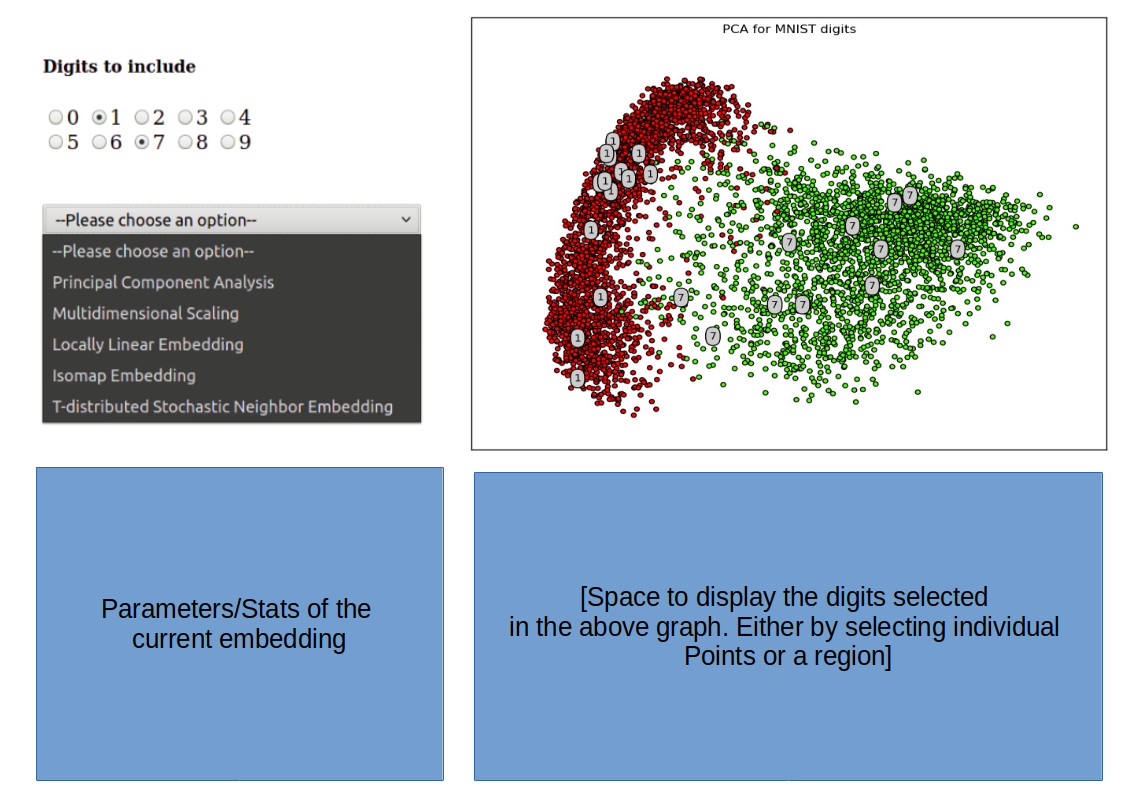
\includegraphics[width=0.45\textwidth]{fig/mockup_va.png} 
    }
    \vspace{3px}
    \fbox{
        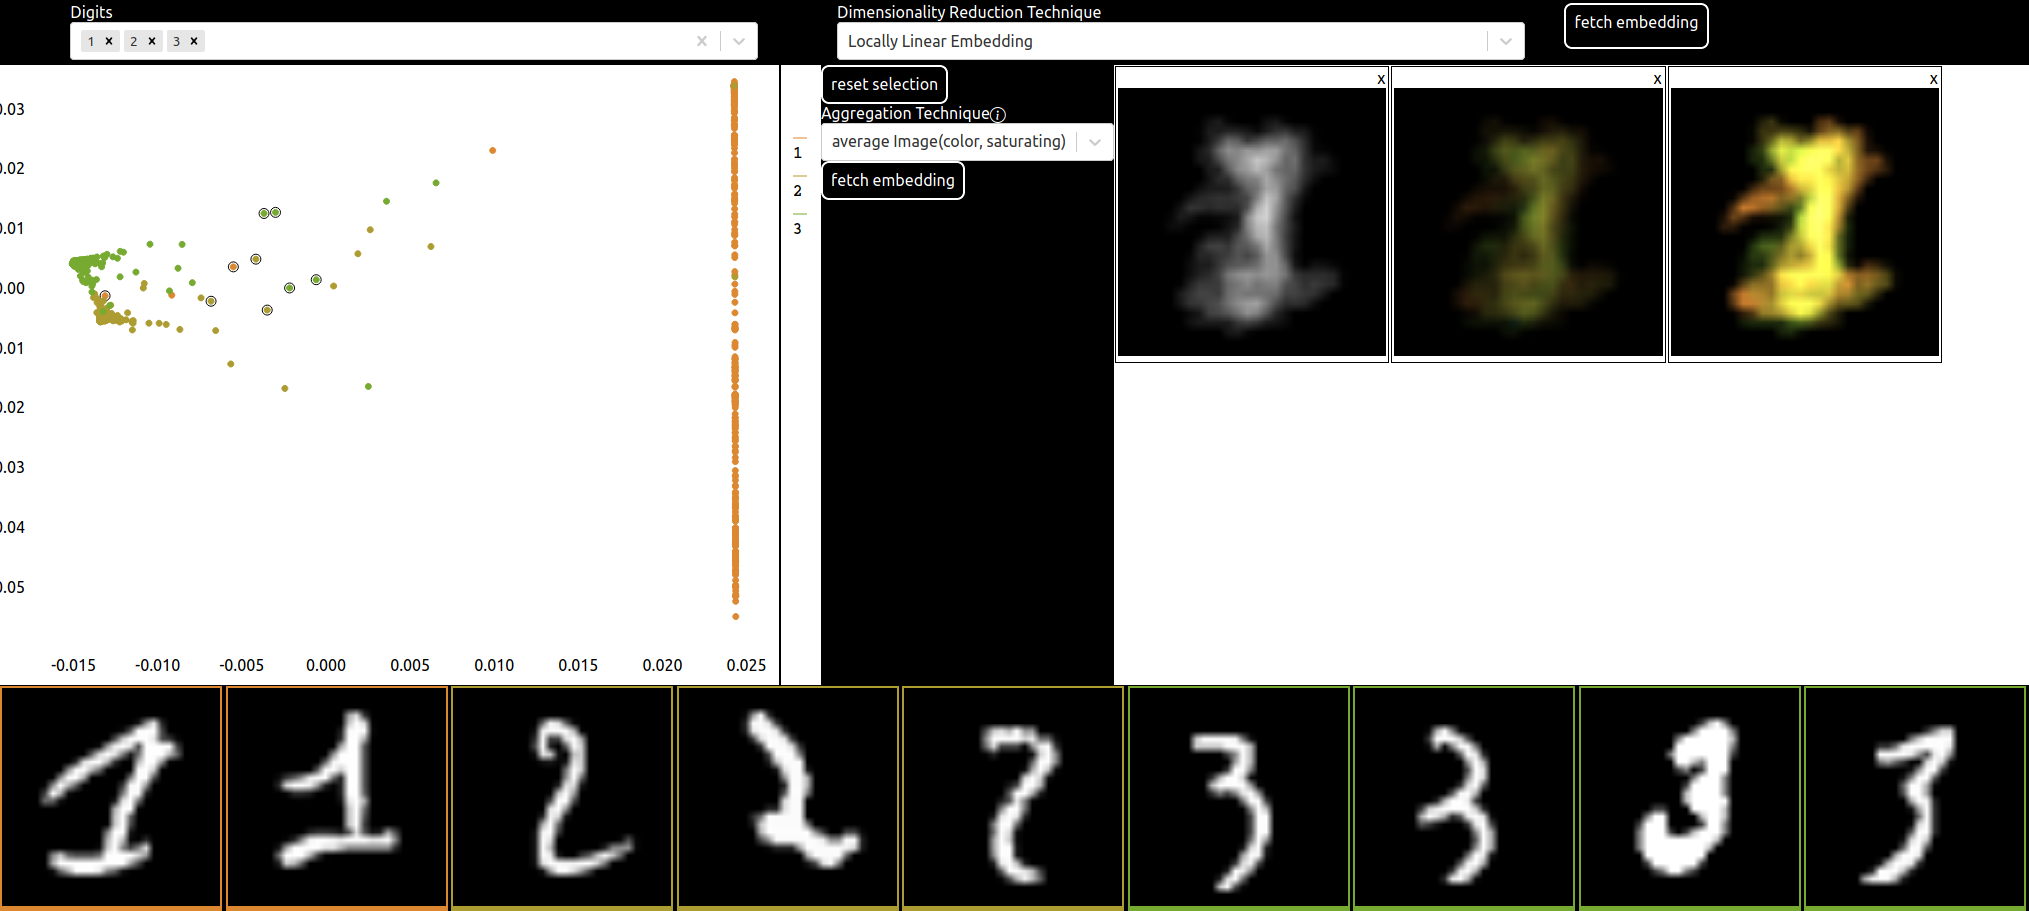
\includegraphics[width=0.45\textwidth]{fig/application_prototype.png}
    }
      \caption{A picture of the proposed mockup vs.  screenshot from the prototype of the application}
    \end{figure}

  \section {Insights}
    \label{insights}

  \section {Demo}
  \section {Conclusion}

  \bibliographystyle{acl_natbib}
  \bibliography{acl2021}

  %\appendix



  \end{document}
